% vim: set spell spelllang=en tw=100 :

\documentclass[letterpaper]{article}

\usepackage[pass]{geometry}

\usepackage{ijcai16}
\usepackage{times}
\usepackage{complexity}
\usepackage{microtype}
\usepackage{amsmath}
\usepackage{amssymb}
\usepackage{amsthm}
\usepackage{cleveref}
\usepackage{tikz}
\usepackage{mathtools}
\usepackage{graphicx}
\usepackage{multicol}
\usepackage[ruled,vlined]{algorithm2e}

% \usepackage{showframe}

\makeatletter\@ifpackageloaded{showframe}{
    % show lines down the middle columns too
    % http://tex.stackexchange.com/questions/16199/test-if-a-package-or-package-option-is-loaded
\newlength\Fcolumnseprule\setlength\Fcolumnseprule{0.4pt}\def\@outputdblcol{%
  \if@firstcolumn\global \@firstcolumnfalse \global \setbox\@leftcolumn \box\@outputbox
  \else
    \global \@firstcolumntrue
    \setbox\@outputbox \vbox{\hb@xt@\textwidth{\hb@xt@\columnwidth{\box\@leftcolumn \hss}%
    \vrule \@width\Fcolumnseprule\hfil{\normalcolor\vrule \@width\columnseprule}
    \hfil\vrule \@width\Fcolumnseprule\hb@xt@\columnwidth {\box\@outputbox \hss}}}\@combinedblfloats\@outputpage
    \begingroup\@dblfloatplacement\@startdblcolumn\@whilesw\if@fcolmade \fi{\@outputpage\@startdblcolumn}\endgroup
  \fi
}}{}
\makeatother

\usetikzlibrary{decorations, decorations.pathreplacing, calc, backgrounds}

\definecolor{uofgsandstone}{rgb}{0.321569, 0.278431, 0.231373}
\definecolor{uofglawn}{rgb}{0.517647, 0.741176, 0}
\definecolor{uofgcobalt}{rgb}{0, 0.615686, 0.92549}
\definecolor{uofgpumpkin}{rgb}{1.0, 0.72549, 0.282353}
\definecolor{uofgthistle}{rgb}{0.584314, 0.070588, 0.447059}

\newcommand{\citet}[1]{\citeauthor{#1} \shortcite{#1}}
\newcommand{\citep}[1]{\cite{#1}}

\theoremstyle{definition}
\newtheorem{proposition}{Proposition}
\newtheorem{corollary}{Corollary}

% cref style
\crefname{figure}{Figure}{Figures}
\Crefname{figure}{Figure}{Figures}

% http://tex.stackexchange.com/questions/22100/the-bar-and-overline-commands
\newcommand{\shortoverline}[1]{\mkern 1.5mu\overline{\mkern-1.5mu#1\mkern-1.5mu}\mkern 1.5mu}


% Maths operators
\newcommand{\paths}{\operatorname{paths}}
\newcommand{\lessnonind}[1]{\prescript{}{#1}{\rightarrowtail}\ }
\newcommand{\lessind}[1]{\prescript{}{#1}{\hookrightarrow}\ }
\newcommand{\lessmap}[1]{\prescript{}{#1}{\mapsto}\ }
\newcommand{\lesspreceq}[1]{\prescript{}{#1}{\preceq}\ }
\newcommand{\V}{\operatorname{V}}
\newcommand{\N}{\operatorname{N}}
\newcommand{\nds}{\operatorname{S}}
\newcommand{\loopcomp}[1]{\oset[.1ex]{\multimap}{#1}}
% to do comments
\usepackage{color}
\newcommand{\todo}[1]{{\color{red} {?? [}{#1}{]}}}

\makeatletter
\newcommand{\oset}[3][0ex]{%
  \mathrel{\mathop{#3}\limits^{
    \vbox to#1{\kern-2\ex@
    \hbox{$\scriptstyle#2$}\vss}}}}
\makeatother

\title{Between Subgraph Isomorphism and Maximum Common Subgraph}

\author{Ruth Hoffmann \and Ciaran McCreesh\thanks{This work was supported by the Engineering and Physical Sciences
Research Council [grant number EP/K503058/1]} \and Craig Reilly\thanks{This work was supported by the Engineering and Physical Sciences Research Council [grant number EP/M506539/1]} \\
University of Glasgow, Glasgow, Scotland \\
ruth.hoffmann@glasgow.ac.uk \and \{c.mccreesh.1,c.reilly.2\}@research.gla.ac.uk}

\pdfinfo{
    /Title (Between Subgraph Isomorphism and Maximum Common Subgraph)
    /Author (Ruth Hoffmann and Ciaran McCreesh and Craig Reilly)
}

\begin{document}

\maketitle

\begin{abstract}
    \todo{anonymise abstract}
    When a small pattern graph does not occur inside a larger target graph, we can ask how to find
    ``as much of the pattern as possible'' inside the target graph. In general, this is known as the maximum
    common subgraph problem, which is much more computationally challenging in practice than
    subgraph isomorphism. We introduce a restricted alternative, where we ask if all but $k$
    vertices from the pattern can be found in the target graph. This allows for the development of
    slightly weakened forms of certain invariants from subgraph isomorphism which are based upon degree and
    number of paths.  We show that when $k$ is small, weakening the invariants still retains much of
    their effectiveness. We are then able to solve this problem on the standard SIP problem
    instances used to benchmark subgraph isomorphism algorithms, despite these instances being
    too large for current maximum common subgraph algorithms to handle.
\end{abstract}
\todo{try code on MCS instances}
\section{Introduction}
\todo{talk about subgraph isomorphism applications, particularly vision}
\todo{talk about reformulating}
The subgraph isomorphism problem is to find a copy of a small \emph{pattern} graph inside a larger
\emph{target} graph. It comes in two forms: in the non-induced variant, edges must be mapped to
edges, but the target may have ``extra edges'', whilst in the induced variant, non-edges may only be
mapped to non-edges. When a pattern cannot be found, we may wish to be given a result which maps as
many vertices of the pattern into the target as possible. In the induced case, this is known as the
maximum common induced subgraph problem (we discuss the non-induced case below). However, although
recent subgraph isomorphism algorithms are comfortable working with graphs with thousands of
vertices, the state of the art for the maximum common subgraph problem becomes computationally
infeasible at only 35 vertices when working with unlabelled graphs
\citep{DBLP:conf/cp/McCreeshNPS16}. This is largely because strong inference, based upon the degrees
of vertices \citep{DBLP:journals/ai/Solnon10} and the distances or paths between them
\citep{DBLP:conf/cp/AudemardLMGP14,DBLP:conf/cp/McCreeshP15}, is possible with subgraph isomorphism,
but not maximum common subgraph, and so the state space in the former is much more restricted,
whilst filtering during search is vastly stronger.

In this work we discuss an intermediate problem, where we must map all but $k$ vertices of the
pattern graph into the target. We show that if $k$ is reasonably small (say, between 1 and 5), then
weakened forms of degree and path based filterings are still effective in pruning the initial search
space and in providing additional constraints respectively. We then show that combining these
techniques leads to a practical algorithm which can scale to work with the families of graphs
commonly used to benchmark subgraph isomorphism algorithms: depending upon the benchmark family, in
a substantial portion of ??; in ?? more cases, we can at least obtain an upper bound.

\subsection{Definitions and Notations}

A non-induced subgraph isomorphism from a graph $P$ to a graph $T$ is an injective mapping $P
\rightarrowtail T $ which maps adjacent vertices to adjacent vertices. An induced subgraph
isomorphism $P \hookrightarrow T$ additionally maps non-adjacent vertices to non-adjacent vertices.
We define a $k$-less-subgraph isomorphism from $P$ to $T$ to be a subgraph isomorphism from all but
$k$ vertices of $P$ to $T$; this may be non-induced or induced, written $P \lessnonind{k} T$ and $P
\lessind{k} T$ respectively.

The \emph{complement} of a (simple) graph $P$ is the graph $\bar{P}~$.  Adjacent vertices in $P$ are
non-adjacent in $\bar{P}$ while non-adjacent vertices in $P$ are adjacent in $\bar{P}$.  The \emph{loop complement} of a graph $P$ is the graph $\loopcomp{P}$.  The constructcion of $\loopcomp{P}$ is similar to that of $\bar{P}~$, however whenever a vertex has a loop in $P$ it does not in $\loopcomp{P}$ and vice versa.  When solving an induced subgraph isomorphism problem we make use of the loop complement; we care about mapping vertices with loops to vertices with loops, and edges without loops to vertices without loops.  (Although when we filter by paths we make use of the complement rather than the loop complement.)  The following proposition follows directly from the definitions.

\begin{proposition}\label{prop:comp}
Let $i$ be an assignment of $T$ vertices to $P$ vertices.  Then $i$ satisfies the definition of $P
\hookrightarrow T$ if and only if $i$ satisfies both the definition of $P \rightarrowtail T$ and
of $\loopcomp{P} \rightarrowtail \loopcomp{T}$.
Similarly, $i$ satisfies the definition of $P
\lessind{k} T$ if and only if $i$ satisfies both the definition of $P \lessnonind{k} T$ and of
$\loopcomp{P}
\lessnonind{k} \loopcomp{T}$.
\end{proposition}

A common induced subgraph of graphs $G$ and $H$ is a graph $P$, together with two induced subgraph
isomorphisms to $G$ and $H$; a maximum common induced subgraph is a common induced subgraph with as
many vertices as possible. An induced $k$-less subgraph isomorphism $P \lessind{k} T$ is equivalent
to a common induced subgraph of $P$ and $T$ with $\left|\V(P)\right| - k$ vertices.

If defined similarly, a maximum common non-induced subgraph would allow us to select every vertex in
the smaller of the two graphs, and none of the edges. It is therefore traditional to change the
objective to maximise the number of edges selected, rather than vertices, when a non-induced common
subgraph is sought---this problem is usually called the maximum common \emph{partial} subgraph
problem instead. However, this is not what we will be discussing in this paper: maximum common
subgraph problems are symmetric in their inputs, but when discussing the non-induced case we are
allowing extra edges only in the target graph, not in the pattern.

\todo{is this example graph still needed?? yes, Patrick likes pictures}

\subsection{Constraint Models and Algorithms}

For both subgraph isomorphism and maximum common subgraph, constraint-based models are the best
approach (although constraint programming toolkits are not used, to facilitate better memory layouts
and propagation queues). For both problems, we create a variable for each vertex in the pattern
graph (the smaller graph, in the case of maximum common subgraph), with domains ranging over the
vertices in the target graph (the larger graph). For maximum common subgraph, each domain is given
an additional $\bot$ value, meaning ``unmapped''.

We also have constraints for adjacency and non-adjacency. For the maximum common subgraph case,
$\bot$ is ignored.

In our algorithm we make use of \cref{prop:comp} by seeking an $i$ which simultaneously satisfies $P
\rightarrowtail T$ and $\bar{P} \rightarrowtail \bar{T}$ when searching for an induced subgraph
isomorphism.  Further, \cref{prop:comp} tells us that every induced subgraph isomorphism is
equivalent to simultaneous non-induced subgraph isomorphisms both $P$ and $T$ as well as their
complements.

All different.

For subgraph isomorphism, we can also do domain filtering at the top of search. We discuss this in
\cref{section:degreefiltering}. Additional constraints, discuss this in \cref{section:pathfiltering}.

?? Also the clique encoding.

?? Explain effectively-unit domain, multiple $\bot$ values.

\subsection{Experimental Setup}

We perform our experiments on systems with dual Intel Xeon CPU E5-2640 processors with 64GBytes of
RAM, running Ubuntu 14.04. Our algorithm was implemented in C++\footnote{URL removed for anonymous
review}, and source code was compiled using
GCC 5.3.0. We used a timeout of 1,000 seconds for each instance.

For datasets, we use the same 5,725 instances used in a recent work on portfolios of algorithms for
subgraph isomorphism \cite{thelionpaper}. This collection includes randomly generated scale-free
graphs \cite{constraints10}, an assortment of real-world graphs of varying sizes \cite{LV02},
randomly generated graph pairs (using bounded degree, regular mesh, and uniform models; all are
satisfiable), segmented images~\cite{pr15,cviu11}, meshes from modelling 3D objects \cite{cviu11},
and graphs close to the satisfiable-unsatisfiable phase transition
\cite{DBLP:conf/ijcai/McCreeshPT16}; all these instances are available in a simple text
format\footnote{\texttt{http://liris.cnrs.fr/csolnon/SIP.html}}.

?? Using the French code, and the Glasgow clique code.

Note that many of these instances are \emph{much} larger than were used in the recent comparison of
maximum common subgraph algorithms by \citet{DBLP:conf/cp/McCreeshNPS16}: for unlabelled graphs,
they used pairs of graphs with up to 35 vertices in each, whilst our dataset contains patterns with
up to ?? vertices and targets with up to ?? vertices. This causes problems: both the maximum common
subgraph algorithm and the clique encoding require $O(\left|\V(P)\right|^2\left|\V(T)\right|^2)$
memory. For maximum common subgraph, 1,560 of the instances cannot fit in the amount of RAM we have
available---we treat these instances as having timed out. The situation for the clique encoding is
even worse, and 3,653 of these instances do not fit in RAM. In contrast, the approach we discuss
here requires only $O(\left|\V(P)\right|^2\left|\V(T)\right|)$ space (which would still be a problem
on some desktop machines, but not on our server hardware).

\section{Domain Filtering using Degrees}\label{section:degreefiltering}

A non-induced $k$-less-subgraph isomorphism from $P$ to $T$ is equivalent to a subgraph
isomorphism between $P$ and $T$ with $k$ extra universally-adjacent vertices. (However, we can do a
bit better algorithmically.) For induced $k$-less-subgraph isomorphisms, such an approach cannot
work.

Let $p$ be a vertex in a graph $P$, the \emph{degree} of $p$, $\deg(p)$, is the number of vertices
to which it is adjacent

\begin{proposition}
    \label{prop:deg}
    Let $p$ be a vertex in $P$ and $t$ a vertex in $T$. For both non-induced and induced
    $k$-less-subgraph isomorphisms, if $p \lessmap{k} t$ then
    $\deg(p) - k \le \deg(t)$.
\end{proposition}
\begin{proof}
Let $p$ be a vertex in $P$, and $t$ a vertex in $T$, with $p\mapsto t$. Then by the definition of subgraph isomorphisms, $\deg(p) \le \deg(t)$. Let $P'$ be $P$ less $k$ vertices and $p$ a vertex in $P'$. Then
\[
\deg_{P}(p)-k \le \deg_{P'}(p) \le \deg_{P}(p) \le \deg(t). \qedhere
\]
\end{proof}

A vertex $q$ which is adjacent to $p$ is called its \emph{neighbour}.  Let $\N(p) = \{ q \in \V(P) :
 p \text{ and } q \text{ are adjacent }\}$ be the set of neighbours of $p$.  The \emph{neighbourhood
degree sequence} (NDS) of $p$, $\nds(p)$, is the (non-ascending) sequence of degrees of its
neighbours.

Let $S = ( s_1 , \ldots , s_n )$ and $T = ( t_1 , \ldots , t_m)$ be two sequences.  We say that $S
\preceq T$ if $n \leq m$ and $\forall s_i \in S$ there exists a distinct $t_j \in T$ with $s_i \leq
t_j$.  When considering a $k$-less-subgraph isomorphism we say that $S \lesspreceq{k}
T$ if $n - k \leq m$ and $\forall s_i \in S \setminus S_k$, where $S_k$ is a subsequence of $S$
containing up to $k$ members of $S$, there exists a distinct $t_j \in T$ with $s_i - k \leq t_j$.


\begin{proposition}\label{prop:nds}
If $p \lessmap{k} t$, then $\nds(p) \lesspreceq{k} \nds(t)$.
\end{proposition}

\begin{proof}
Let $p \lessmap{k} t$.  Then $\deg(p) - k \leq \deg(q)$, by \cref{prop:deg}, which
implies that $\left|\nds(p)\right| -k \leq \left| \nds(t) \right| $.

Also, $p \lessmap{k} t$ implies that for each $q \in N(p) \setminus P_k$, where $P_k$
is some subset of $P$ with $\left| P_k \right| \leq k$, $q \lessmap{k} u$, where $u \in N(t)$ and
each $u$ is distinct.  Then $\deg(q) - k \leq \deg(u)$, by \cref{prop:deg}.  Hence $\nds(p)
\lesspreceq{k} \nds(t)$.
\end{proof}

Figure\ref{fig:nds} illustrates the three cases possible when filtering by neighbourhood degree
sequence.  Removing the top node causes each entry in $\nds(p)$ to be reduced; removing the
left-middle node removes an entry from $\nds(p)$; and removing either of the connected nodes in the
middle layer causes both the size of $\nds(p)$ to be reduced and an entry in $\nds(p)$ to be reduced.

\begin{corollary}
Since both $\nds(p)$ and $\nds(t)$ are non-ascending, without loss of generality we can replace
$S \setminus S_k$ from the definition of $S \lesspreceq{k} T$ with $S[k, n]$.
\end{corollary}

\begin{proof}
\todo{Sketch?? Let $S_k$ be some elements of the sequence which aren't the first $k$ elements.  Then these elements are less than or equal to the first $k$ elements.}
\end{proof}


\begin{figure}
    \begin{center}
        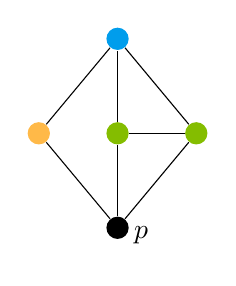
\begin{tikzpicture}[every node/.style={circle, inner sep=1mm}]
            \node[fill=black] (p) {};
            \node[draw=none,right of = p,node distance=3mm,yshift=-1mm] {$p$};
            \node[fill=uofglawn] (n2) [above of = p,node distance=12mm] {};
            \node[fill=uofgpumpkin] (n1) [left of = n2] {};
            \node[fill=uofglawn] (n3) [right of = n2] {};
            \node[fill=uofgcobalt] (q) [above of = n2,node distance=12mm] {};
            \path (p) edge (n1) edge (n2) edge (n3)
                (n1) edge (q)
                (n2) edge (n3) edge (q)
                (n3) edge (q);
        \end{tikzpicture}
        \caption{Example of neighbourhood degree filtering cases}
        \label{fig:nds}
    \end{center}
\end{figure}

?? Talk about iterating, what to do when a vertex disappears from all target graphs.

In \cref{figure:ids} we show that this is useful in practice.

\begin{figure}
    \includegraphics*{gen-graph-ids.pdf}
    \caption{We get domain filtering. Woohoo.}\label{figure:ids}
\end{figure}

\section{Filtering During Search Using Paths}\label{section:pathfiltering}

As well as reasoning about degrees, we can also reason about paths.

A \emph{path} between two vertices $p$ and $q$ is a sequence of edges which can be traversed from $p$ to reach $q$. We define $\paths(p,q,n)$ to be the number of paths of length $n$ between the vertices $p$ and $q$.
%\todo{Define paths}

\begin{proposition}
    Let $p,q \in \V(P)$ and $t,u\in \V(T)$. If $p \lessmap{k} t$ and $q \lessmap{k} u$ then
     $\paths(p, q, 2) - k \le \paths(t, u, 2)$.
\end{proposition}
\begin{proof}
Let $P_{2}$ be the set of all paths of length two between $p$ and $q$,
\begin{align*}
P_{2} = & \{((p,x),(x,q)) : (p,x),(x,q)\in E(P) \} \\
 = & \{((p,x),(x,q)) : x\in \N(p) \text{ and } x\in \N(q) \} \\
 = & \{((p,x),(x,q)) : x\in \N(p)\cap \N(q) \} .
\end{align*}
So $\paths(p,q,2) = \left| \N(p)\cap \N(q) \right|  \leq \deg(p)$.

If we remove up to $k$ vertices from the neighbourhood of $p$, it will impact the intersection of the neighbourhoods of $p$ and $q$, and by Proposition~\ref{prop:deg}, as $p\lessmap{k}t$
\[
\left| \N(p)\cap \N(q)\right| - k \leq \deg(p) - k \leq \deg(t).
\]
As $\left|\N(p)\cap \N(q)\right|\leq \deg(p) \leq \left|\N(t)\cap \N(u)\right|\leq \deg(t)$, we have
\[
\left|\N(p)\cap \N(q)\right| - k \leq \deg(p) - k\leq \left|\N(t)\cap \N(u)\right|\leq \deg(t)
\]
which is
\[
\paths(p, q, 2) - k \leq \paths(t, u, 2). \qedhere
\]
\end{proof}

This leads to the following:

\begin{proposition}
    For a graph $G$, let $G^{n, \ell}$ be the graph with vertex set $\V(G)$. The
    vertices $p$ and $q$ in $G^{n, \ell}$ are adjacent, if there are at least $n$ simple paths of
    length exactly $\ell$ between $p$ and $q$ in $G$. Then any $k$-less-subgraph isomorphism
    $P \lessnonind{k} T$ induces a new $k$-less-subgraph isomorphism
    $P^{n+k, 2}\lessnonind{k} T^{n, 2}$.
\end{proposition}

To allow for fast propagation, we create supplemental graphs for paths of length 2, looking at
counts of 1, 2, and 3 in the target graph (and so counts of $1 + k$ up to $3 + k$ in the pattern).
We then investigate whether this leads to new constraints being generated. By an assignment, we mean
considering mapping a pattern vertex $p$ to a target vertex $t$ (and not $\bot$) which does not
violate any loop constraints. An assignment pair is two assignments with distinct $p$ and distinct
$t$, which we say is permitted if it does not violate any adjacency constraint. We define the
permitted assignment pair ratio to be the proportion of assignment pairs which are permitted.
Finally, we scatter plot the permitted assignment pair ratio with and without supplemental
graphs\footnote{Because of the large sizes of the domains, we randomly sample one million pairs
rather than considering every pair. In some cases, we have nearly a thousand domains, each with nearly
ten thousand values---a complete quadratic calculation involving even a trivial arithmetic operation
on this would take many hours.}. For $k = 0$, we see many points above the $x-y$ diagonal, which
shows that for many instances, we are able to create a substantial number of new constraints at the
top of search; on the other hand, there are also points on the diagonal, which shows that sometimes
this technique provides no benefit. (Occasionally, points fall below the $x-y$ diagonal. This is
because the use of neighbourhood degree sequence reasoning on supplemental graphs can also lead to
increased domain filtering, which could in turn eliminate a higher proportion of forbidden than
permitted assignment pairs.) For $k = 1$ and $k = 2$, the proportion of points above the diagonal
diminishes, but we are still able to create new constraints for many instances. By the time $k = 3$,
most of the benefit is disappearing---although sometimes we are still able to make a difference, and
bear in mind that sometimes adding just one new constrained pair can vastly reduce the search space.

A closer inspection of the raw data shows that for $k = 3$, nearly all of the instances showing a
strong improvement are from the ``LV'' family of graphs.

\begin{figure*}
    \includegraphics*{gen-graph-constraints.pdf}\\[0.1cm]
    \includegraphics*{gen-graph-constraints-induced.pdf}
    \caption{We get new constraints. More woohoo.}\label{figure:constraints}
\end{figure*}

\section{A New Algorithm}

\begin{algorithm*}[tb]
\DontPrintSemicolon
\begin{multicols}{2}
\nl $\FuncSty{klessSubgraphIsomorphism}$ (\\\hspace*{2em}Graph $\mathcal{P}$, Graph $\mathcal{T}$, Int $k$) $\rightarrow$ Bool \;
\nl \Begin{
    \nl \lIf{$\left|\V(\mathcal{P})\right| + k > \left|\V(\mathcal{T})\right|$}{$\KwSty{return}~\KwSty{false}$\label{line:enough}}
    \nl $L \gets \big[ (\mathcal{P},\ \mathcal{T}), (\shortoverline{\mathcal{P}},
        \shortoverline{\mathcal{T}}),$
        \\\hspace*{1.0em}$(\mathcal{P}^{1 + k,2},\ \mathcal{T}^{1,2}), (\mathcal{P}^{2 + k,2},\
    \mathcal{T}^{2,2}), (\mathcal{P}^{3 + k,2},\ \mathcal{T}^{3,2}) \big]$ \;
    \nl \ForEach{$v \in \V(\mathcal{P})$}{
        \nl $D_v \gets \V(\mathcal{T})$\;
        \nl \ForEach{$(P,\,T) \in L$}{
            \nl $D_v \gets \{ w \in D_v : $ \\
            \hspace*{4em}$v \sim_P v \Rightarrow w \sim_T w~\wedge$ \\
            \hspace*{4em}$\nds_P(v) \lesspreceq{k} \nds_T(w)\}$ \;
        }
        \nl $D_v \gets D_v \cup k~\textnormal{distinct wildcard values}$
    }
    \nl \lIf{\FuncSty{propagate}(D)}{$\KwSty{return}~\FuncSty{search}(L, D, k)$}
    \nl \lElse{$\KwSty{return}~\KwSty{false}$}
}
\bigskip
\nl $\FuncSty{search}$ (GraphPairs $L$, Domains $D$, Int $k$) $\rightarrow$ Bool \;
\nl \Begin{
    \nl \lIf{$D = \emptyset$}{$\KwSty{return}~\KwSty{true}$}
    \nl $D_v \gets \textnormal{the smallest domain in}~D$ \;
    \nl \ForEach {$v' \in D_v~\textnormal{ordered by static degree in}~\mathcal{T}$\label{line:parforeach}}{
        \nl \If{$v'$ \textnormal{is not the first wildcard we have tried}}{
            \nl \KwSty{continue} \;
        }
        \nl $D' \gets \FuncSty{clone}(D)$ \;
        \nl $D'_v \gets \{ v' \} $ \;
        \nl \If{\FuncSty{propagate}(D')}{
            \nl \If{$\FuncSty{search}(L, \{ D \in D' : \left|D\right| > 1 \}, k)$}{
                \nl $\KwSty{return}~\KwSty{true}$ \;
            }
        }
    }
}
\bigskip
\nl $\FuncSty{propagate}$ (GraphPairs $L$, Domains $D$) $\rightarrow$ Bool \;
\nl \Begin{
    \nl \While{\KwSty{true}}{
        \nl \If{\textnormal{no effectively-unit domains (treating all wildcard values as a single
        value) remain}}{
            \nl \If{$\KwSty{not}~\FuncSty{allDifferent}(D)$}{
                \nl $\KwSty{return}~\KwSty{false}$ \;
            }
        }
        \nl \If{\textnormal{no effectively-unit domains remain}}{
            \nl $\KwSty{return}~\KwSty{true}$ \;
        }
        \nl $D_v \gets \textnormal{an effectively-unit domain from}~D$ \;
        \nl $v' \gets $ the single value in $D_v$, or an arbitrary wildcard value if there is more
        than one \;
        \nl \ForEach{$D_w \in D \setminus \{ D_v \}$}{
            \nl $D_w \gets D_w \setminus \{ v' \}$ \label{line:removev} \;
            \nl \ForEach{$(P,\,T) \in L$}{
                \nl \If{$v \sim_P w$}{
                    \nl $D_w \gets D_w \cap \left(\N_T(v') \cup \textnormal{wildcards}\right)$
                }
            }
            \nl \lIf{$D_w = \emptyset$}{$\KwSty{return}~\KwSty{false}$}
        }
    }
}
\bigskip
\nl $\FuncSty{allDifferent}$ (Domains $D$) $\rightarrow$ Bool \;
\nl \Begin{
\nl $(F,\,H,\,A,\,n) \gets (\emptyset,\,\emptyset,\,\emptyset,\,0)$ \;
\nl \ForEach{$D_v \in D$ \textnormal{from smallest to largest\label{line:eachdomain}}}{
    \nl $F \gets F \cup \{ v \}$ \;
    \nl $D_v \gets D_v \setminus H$ \label{line:elimhall} \;
    \nl $(A,\,n) \gets (A \cup D_v,\,n + 1)$ \label{line:acc} \;
    \nl \lIf{$D_v = \emptyset~\KwSty{or}~\left|A\right| < n$}{$\KwSty{return}~\KwSty{false}$\label{line:failhall}}
    \nl \lIf{$\left|A\right| = n$}{$(H,\,A,\,n) \gets (H \cup A,\,\emptyset,\,0)$\label{line:hall}}
}
\nl $\KwSty{return}~\KwSty{true}$ \;
}
\end{multicols}
\vspace*{0.4cm}% bug in algorithm2e + multicol: incorrect space left above the vertical line
\caption{An algorithm for the $k$-less subgraph isomorphism problem.}
\label{algorithm:sip}
\end{algorithm*}

\section{Empirical Evaluation}

\begin{figure}
    \includegraphics*{gen-graph-runtimes.pdf}
    \caption{Look how amazing our stuff is.}\label{figure:runtimes}
\end{figure}

\subsection{Induced}

What proportion of instances are actually satisfiable as $k$ increases?

\begin{figure}
    \includegraphics*{gen-graph-which-k-by-family.pdf}
    \caption{There are satisfiable instances for small values of $k$. Yay.}\label{figure:which-k}
\end{figure}

\subsection{Non-Induced}

What proportion of instances are actually satisfiable as $k$ increases?

\subsection{Solving from the Top Down}

\begin{figure}
    \includegraphics*{gen-graph-versus-cp.pdf}
    \caption{A righteous spanking.}\label{figure:versus-cp}
\end{figure}

\section{Conclusion}

\section*{Acknowledgements}

We're not going to thank anyone, no, no.  Thanks to Frances for making us less smelly throughout the writing of the paper (by thieving toiletries from a fancy hotel).

\bibliographystyle{named}
\bibliography{paper}

\end{document}
